% TikZ content only. Intended to be included from benchmark-construction-slide.tex.
\begin{tikzpicture}[
  x=1cm,
  y=1cm,
  image/.style={inner sep=0pt},
  sidecaption/.style={font=\scriptsize\bfseries, align=center, text=black},
  note/.style={font=\tiny, align=center, text=black!70},
  flow/.style={-{Latex[length=2.3mm]}, line width=0.85pt, draw=blue!65!black},
  softflow/.style={-{Latex[length=2.2mm]}, line width=0.75pt, draw=blue!45!black},
]

% 2 x 2 layout:
% NW: EURADCLIM, NE: 100 patch locations, SW: 4TU, SE: example patch.
% All raster panels are intentionally forced to roughly the same square size.

\newcommand{\panelsize}{3.25cm}
\newcommand{\patchsize}{3.65cm}

\node[image] (eurad) at (2.45,4.85)
  {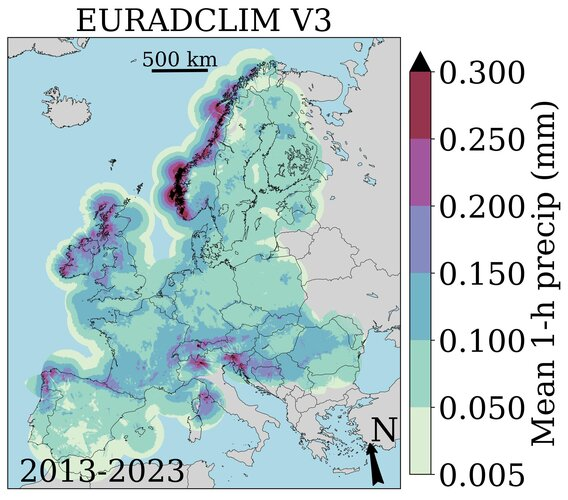
\includegraphics[width=\panelsize,height=\panelsize]{EURADCLIM.jpg}};
\node[sidecaption, anchor=north west] at ([xshift=8mm,yshift=-1mm]eurad.north)
  {\textsuperscript{*}};

\node[image] (locations) at (9.00,4.85)
  {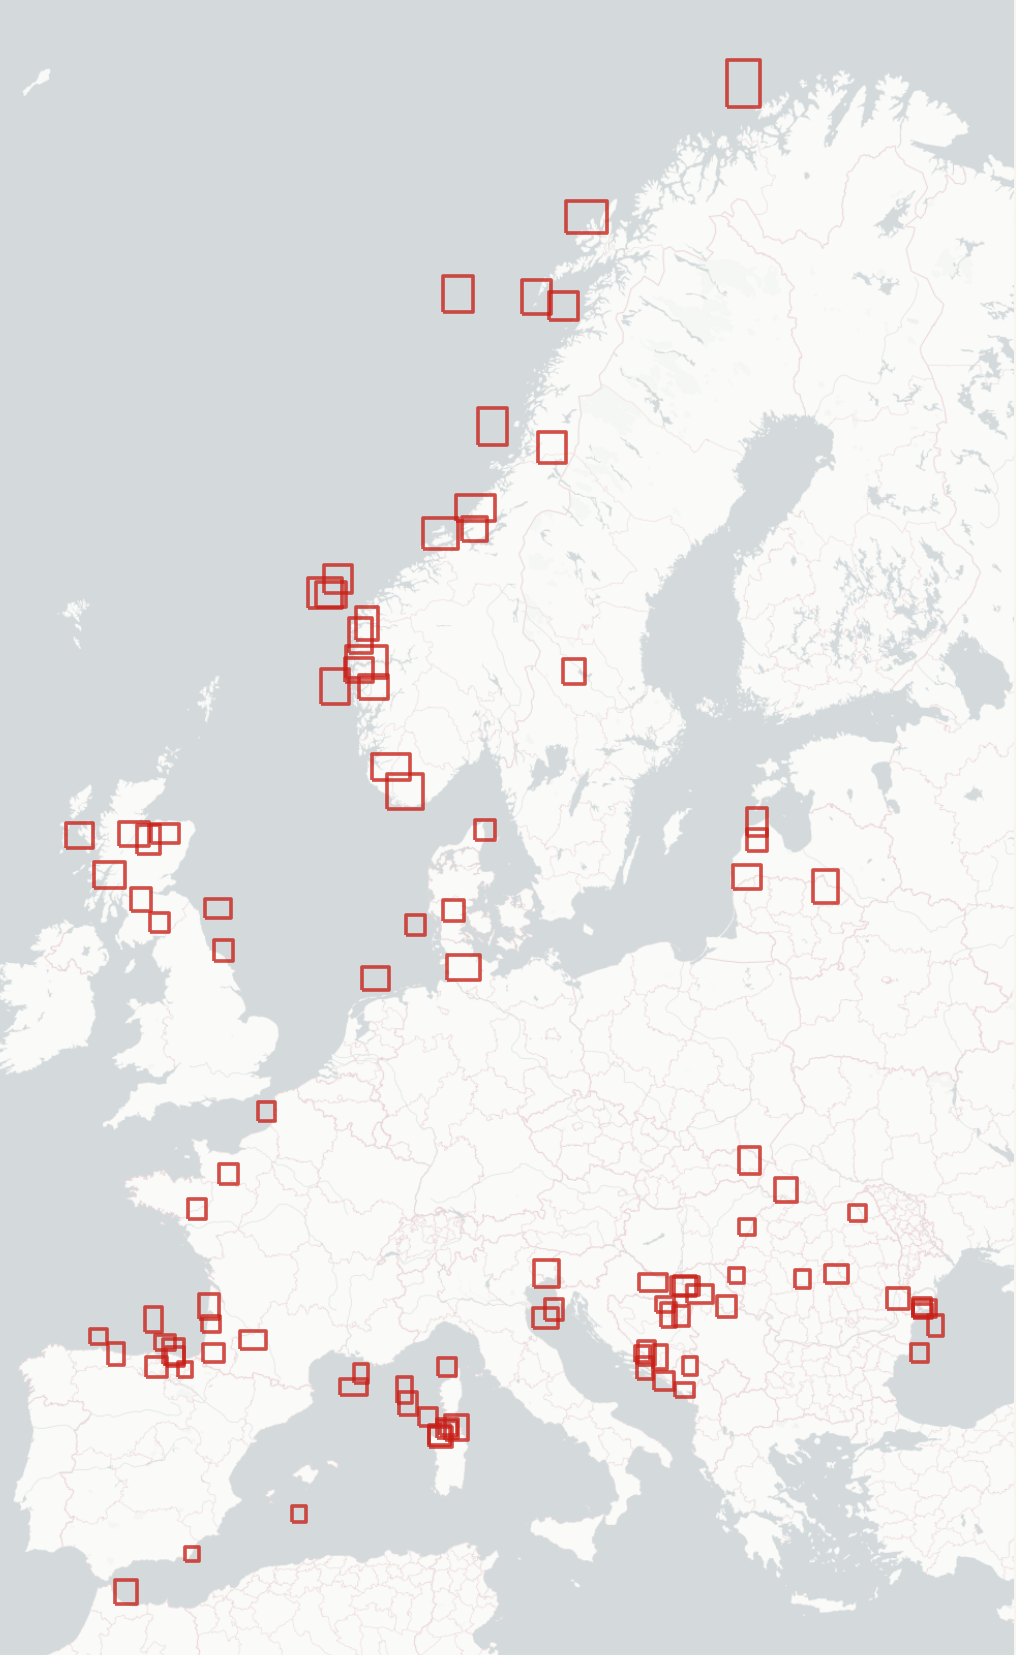
\includegraphics[width=\panelsize,height=\panelsize]{100patches-locations.png}};

\node[image] (links) at (2.45,1.10)
  {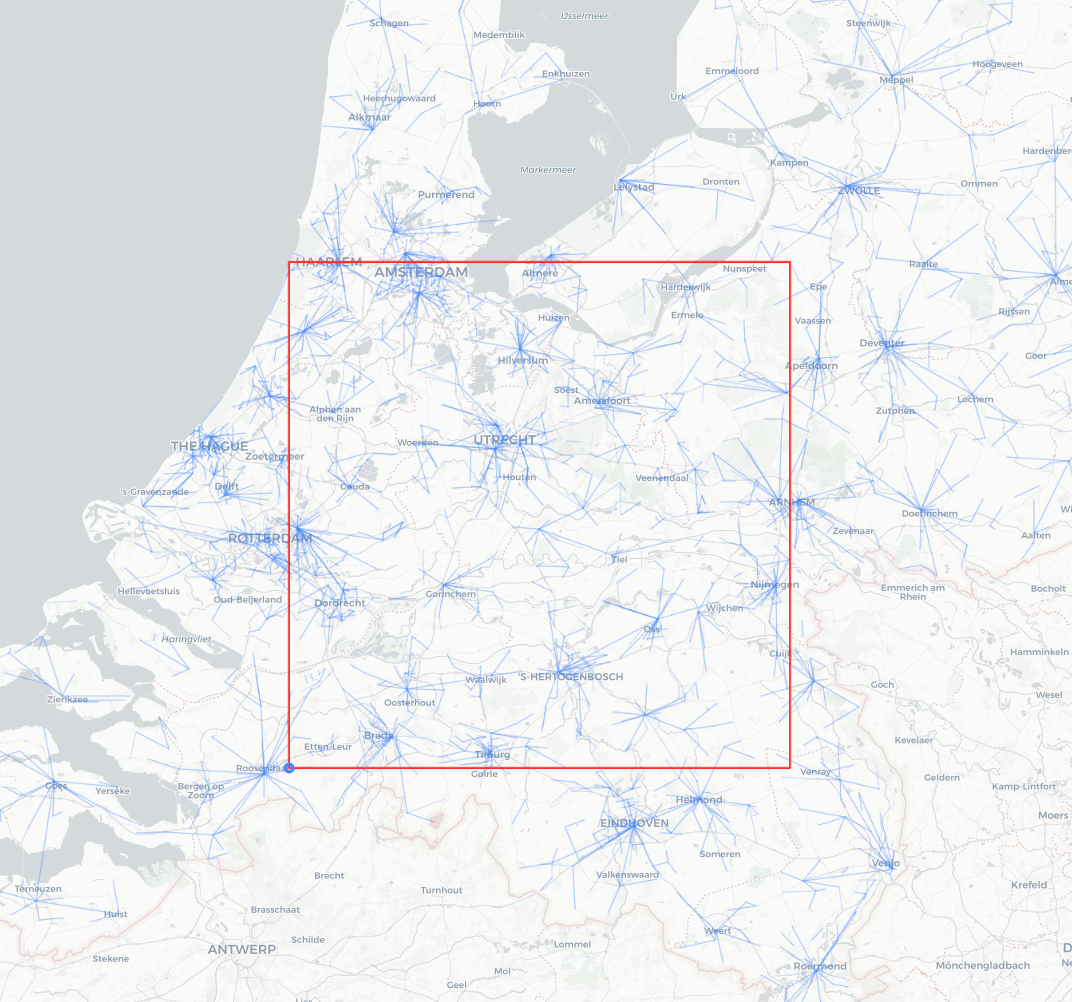
\includegraphics[width=\panelsize,height=\panelsize,trim={248bp 194bp 242bp 223bp},clip]{map-4TU-Links.png}};
\node[sidecaption, anchor=north] at ([yshift=-1mm]links.north)
  {4TU\textsuperscript{\ensuremath{\dagger}}};

% Keep the original top-left corner of the example patch while enlarging it.
\node[image, anchor=north west] (patch) at (7.175,2.725)
  {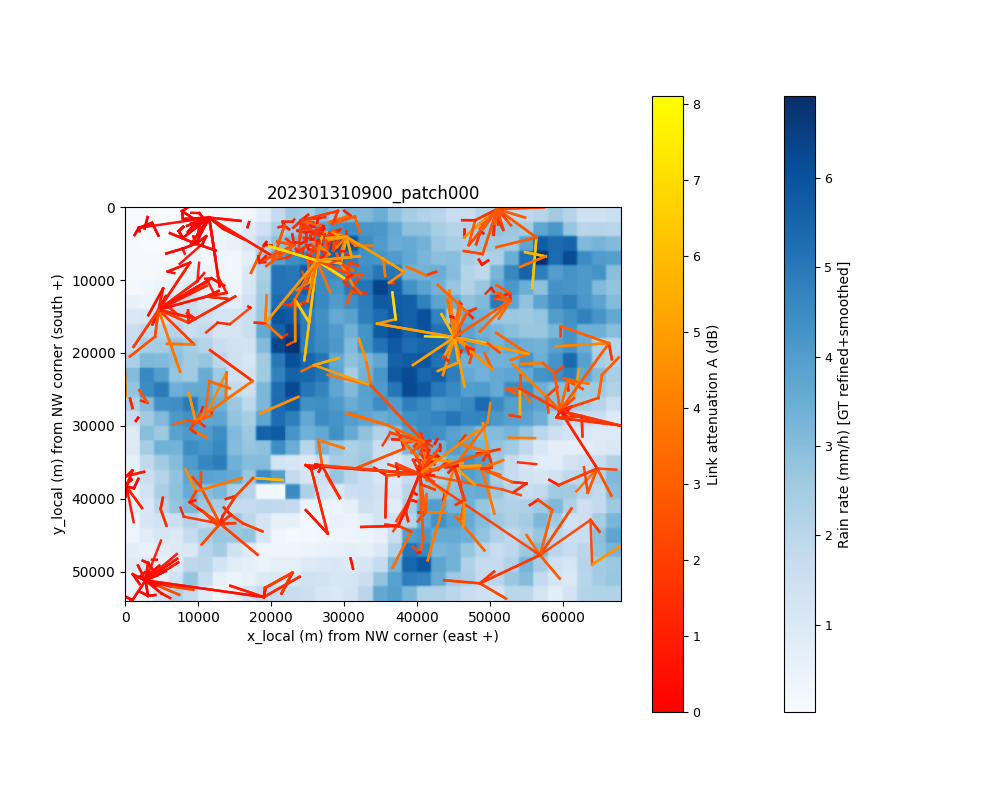
\includegraphics[width=\patchsize,height=\patchsize]{0900_patch000.png}};

% Axis-parallel arrows, each with a single straight segment.
\draw[flow]
  (eurad.east) -- node[note, above, midway] {automatic extraction\\of rain event}
  (locations.west);

\draw[flow]
  (locations.south) -- node[note, left=1.5mm, midway, anchor=east, align=center] {link atten\\=\\ITU(rain)}
  ([yshift=-6mm]patch.north);

\draw[softflow]
  (links.east |- patch.west) -- node[note, above, midway] {clip link geometry\\+ parameters}
  (patch.west);

% Source line inside the slide canvas, not as a Beamer footer.
\node[anchor=south west, font=\fontsize{4.5}{4.8}\selectfont, text=black!65, align=left] at (0.0,-1.05)
  {\textsuperscript{*} EURADCLIM rainfall fields: Overeem et al. (2023), KNMI.};
\node[anchor=south east, font=\fontsize{4.5}{4.8}\selectfont, text=black!65, align=right] at (11.2,-1.05)
  {\textsuperscript{\ensuremath{\dagger}} CML data: Overeem et al. (2016), 4TU.ResearchData. Attenuation: ITU-R P.838-3.};

\end{tikzpicture}
